\documentclass[a4paper,10pt]{exam}

\usepackage[utf8]{inputenc}
\usepackage[cyr]{aeguill}
\usepackage[francais]{babel}
\usepackage{fullpage}
\usepackage{amsmath}
\usepackage{array}
\usepackage{tikz}
\input kvmacros
\usetikzlibrary{arrows,shapes,trees,patterns,fit,backgrounds,%
decorations.pathreplacing,chains,calc,decorations.pathmorphing,matrix,circuits.logic.CDH}


\ifthenelse{\equal{\detokenize{correction}}{\jobname}}
{\printanswers}
{\noprintanswers}

\title{Architecture des ordinateurs - TD 08}

\author{}
\date{}

\begin{document}
\maketitle

\section{Logique asynchrone}
\subsection{Bascule SR}

Voici le diagramme d'une bascule SR ainsi que son implémentation avec deux
portes NOR.

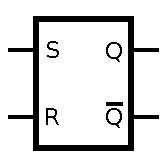
\includegraphics[width=2cm]{SRflipflop} \hspace{1cm}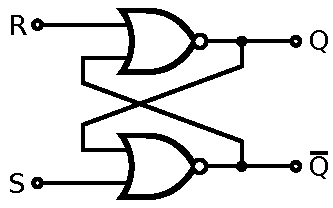
\includegraphics[width=4cm]{SR-design}

\begin{enumerate}
  \item Écrire la table de vérité pour $R$,$S$,$Q$ et $\overline{Q}$. Attention
    certains états peuvent être indéterminés.
\begin{solution}
\begin{tabular}{cc|cc}
  $S$&$R$&$Q$&$\overline{Q}$\\
  \hline
  0 & 0  & Q & $\overline{Q}$ \\
  0 & 1  & 0 & 1 \\
  1 & 0  & 1 & 0 \\
  1 & 1  & 0 & 0
\end{tabular}

Attention le dernier état est interdit:
\begin{itemize}
  \item Il viole la convention $Q = \textrm{not} \overline{Q}$
  \item Le passage de 1,1 à 0,0 peut mettre la bascule dans un état indéterminé.
\end{itemize}
\end{solution}


  \item Soit $Q$ l'état actuel d'une bascule et $Q^{+}$ l'état suivant. Écrire
    la table de vérité reliant $Q$,$Q^{+}$,$S$ et $R$.

  \item Trouver l'équation logique minimale pour cette table de vérité
    ($f(Q,S,R) = Q^{+}$). (Utilisez la méthode de votre choix : Karnaugh, etc.)
    Cette équation est l'équation caractéristique de la bascule SR.

\begin{solution}
\begin{tabular}{cc|cc}
  $Q$&$Q^{+}$&S&R\\
  \hline
  0  & 0     &0&X\\
  0  & 1     &1&0\\
  1  & 0     &0&1\\
  1  & 1     &X&0
\end{tabular}
$$ Q^{+} = \overline{R} (Q + S) $$
\end{solution}

  \item Expliquer le fonctionnement de la bascule SR avec des mots.

\begin{solution}
  Dans une bascule SR, soit le bit d'entr\'ee S (pour Set) est \`a 1, ce qui force le passage
  \`a 1 de la sortie Q, soit le bit d'entr\'ee R (pour Reset) est \`a 1, ce qui force le passage
  \`a 0 de Q. Les entr\'ees S et R ne peuvent \^etre mises \`a 1 simultan\'ement. Si elles sont
  toutes les 2 \`a 0, la sortie conserve son \'etat pr\'ec\'edent.
\end{solution}
\end{enumerate}


\subsection{Bascule GL}
\begin{enumerate}
  \item Une bascule GL se comporte de la manière suivante: si $G = 0$, la
    bascule ne change pas d'état. Si $G = 1$, le prochain état de la bascule
    est égal à la valeur de L. Concevez une bascule GL à partir d'une bascule
    SR.

    \begin{solution}

      La bascule GL a pour équation caractéristique :
      $$ Q^{+} = \overline{G}.Q + G.L $$

      Construisons la table de vérité d'une bascule GL.
      On rajoute alors les colonnes S et R, que l'on remplit de manière
      à satisfaire $Q \rightarrow Q^{+}$ (il suffit de consulter la table
      de caractéristique de la bascule SR).

\begin{verbatim}
         G L Q Q+| S R
         --------+-----
         0 0 0 0 | 0 X
         0 0 1 1 | X 0
         0 1 0 0 | 0 X
         0 1 1 1 | X 0
         1 0 0 0 | 0 X
         1 0 1 0 | 0 1
         1 1 0 1 | 1 0
         1 1 1 1 | X 0
\end{verbatim}

      On veut fabriquer une bascule GL à partir d'une bascule SR.
      Il faut donc trouver les fonction $S(G,L,Q)$ et $R(G,L,Q)$.
      Pour cela on peut utiliser la méthode de Karnaugh:

\begin{verbatim}
   S                   R
      LQ\G 0  1           LQ\G 0  1
      00   0  0           00   X |X|
      01   X  0           01   0 |1|
      11   X |X|          11   0  0
      10   0 |1|          10   X  0
\end{verbatim}

$$ S = GL \textrm{ et } R = G\overline{L} $$

      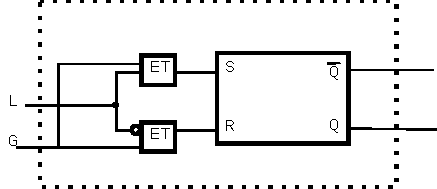
\includegraphics[width=6cm]{TD8-GL}
    \end{solution}

\end{enumerate}

\section{Logique synchrone}
\subsection{Bascule D}

La bascule D est commandée par les entrées $D$ et un signal d'horloge $CK$
(figuré par un petit triangle).
La table de vérité pour la bascule D est donnée ci-dessous:

\begin{center}
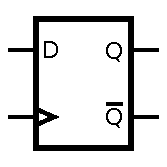
\includegraphics[width=2cm]{Dflipflop}\begin{tabular}{c|c|c|c}
  $CK$&$D$&$Q$&$Q^{+}$\\
  \hline
  $\nearrow$&0  & 0     &0\\
  $\nearrow$&0  & 1     &0\\
  $\nearrow$&1  & 0     &1\\
  $\nearrow$&1  & 1     &1\\
  X         &X  & 1     &1\\
  X         &X  & 0     &0\\
\end{tabular}
\end{center}

\begin{enumerate}
  \item Donner son équation caractéristique et expliquer son fonctionnement avec
    des mots.
\end{enumerate}

\begin{solution}
  $$ Q^{+}= D . (CK\nearrow)$$
\end{solution}

\subsection{Bascule JK}

La bascule JK est commandée par les entrées $J$, $K$ et un signal d'horloge
$CK$.

Lorsque le signal d'horloge est en front montant:

\begin{minipage}{0.4\textwidth}
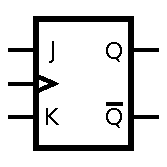
\includegraphics[width=2cm]{JKflipflop}
\end{minipage}
\begin{minipage}{0.4\textwidth}
\begin{itemize}
  \item $JK=00$ : hold, rien ne change
  \item $JK=01$ : reset, $Q^{+}= 0$
  \item $JK=10$ : set, $Q^{+}= 1$
  \item $JK=11$ : toggle, $Q^{+} = \overline{Q}$
\end{itemize}
\end{minipage}

\begin{enumerate}
  \item Donner l'équation caractéristique de JK sur un front montant de $CK$.
    \begin{solution}
      $$Q^{+} = J\overline{Q} + \overline{K}Q$$
    \end{solution}
\end{enumerate}

\subsection{Exercices}


\begin{enumerate}
  \item Fabriquez une bascule JK avec horloge en utilisant uniquement une
    bascule D et des portes logiques élémentaires.
    \begin{solution}
      $$ D = J\overline{Q} + \overline{K}Q$$

      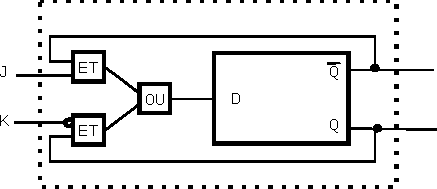
\includegraphics{TD8-JK}
    \end{solution}

  \item Une bascule T se comporte de la manière suivante: si $T = 1$ lors du
    front montant de $CK$ alors $Q^{+} = \overline{Q}$. Comment construire
    une bascule T à partir d'une bascule D ?

    \begin{solution}
      $$ Q = T.\overline{Q} + \overline{T}.Q = T \oplus Q $$

      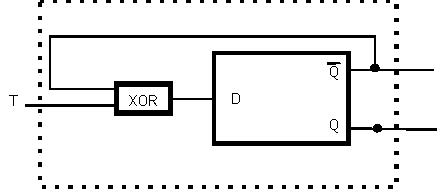
\includegraphics{TD8-T}
    \end{solution}
    \begin{center}
      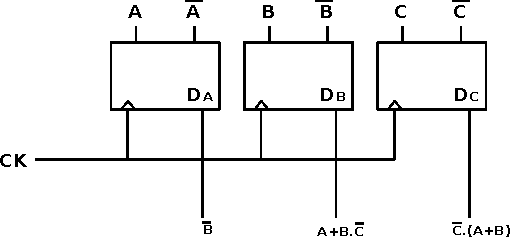
\includegraphics[width=6cm]{TD8-4}
    \end{center}

  \item Donner le chronogramme des variables $CK,A,B,C,D_A,D_B,D_C$. Au temps
    zéro, $A=B=C=0$

    \begin{solution}
      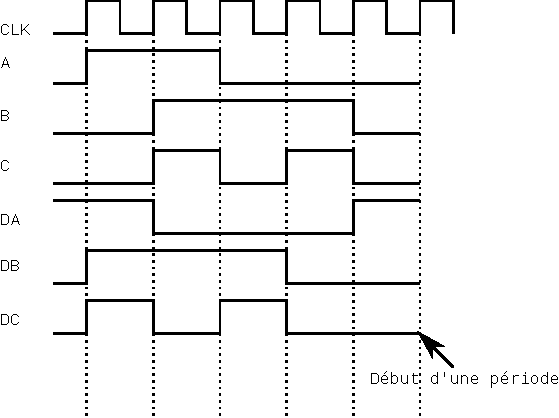
\includegraphics{TD8-chrono}

      Pour trouver les sorties A,B,C au top $T$ on regarde les entrées DA,DB,DC
      au top $T-1$.
    \end{solution}

\end{enumerate}
\section{Compteurs}
\begin{enumerate}
\item Concevoir un compteur qui compte en binaire de 0 à 7. À chaque pas
  d'horloge, le compteur est incrémenté de 1.
  \begin{enumerate}
  \item Concevez un incrémenteur 3 bits avec trois entrées $A=a_2a_1a_0$ et
    trois sorties $B=b_2b_1b0$ de telle sorte que $B = A + 1 [8]$.

\begin{solution}
  On écrit la table de vérité de l'incrémenteur:
\begin{verbatim}
  a2 a1 a0 | b2 b1 b0
   0  0  0 |  0  0  1
   0  0  1 |  0  1  0
   0  1  0 |  0  1  1
   0  1  1 |  1  0  0
   1  0  0 |  1  0  1
   1  0  1 |  1  1  0
   1  1  0 |  1  1  1
   1  1  1 |  0  0  0
\end{verbatim}
En utilisant la méthode de Karnaugh ou de Quine - Mc Cluskey on trouve:
$$ b_2 = \overline{a_2}.a_1.a_0 + a_2(\overline{a_1} + \overline{a_0}) $$
$$ b_1 = a_1 \oplus a_0 $$
$$ b_0 = \overline{a_0} $$

Ce qui nous permet de réaliser le circuit de l'incrémenteur.
\end{solution}

  \item Implémentez le compteur séquentiel en utilisant des bascules D et
    l'incrémenteur précédent. Lorsque le compteur atteint 7, au front d'horloge
    suivant il revient à 0.

  \item Comment rajouter un bouton reset pour remettre le compteur à zéro ?

\begin{solution}
  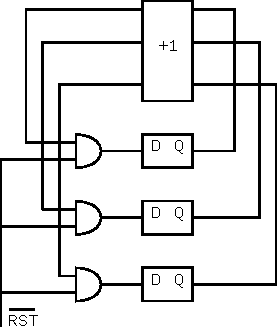
\includegraphics{TD8-inc}
\end{solution}

\end{enumerate}


  \item Concevoir un compteur qui produit la séquence suivante:
    $$0000,1000,1100,1010,1110,0001,1001,1101,1011,1111,0000, \dots$$

    \begin{itemize}
      \item en utilisant des bascules T.
        \begin{solution}
          La méthode se décompose en trois étapes:
          \begin{itemize}
            \item On écrit la table de vérité reliant l'état courant et l'état
              suivant. Ici on a quatre bits d'états (compteur 4 bits), donc
              on va écrire la table pour $QA,QB,QC,QD$ et $QA^+$,$QB^+$,$QC^+$,$QD^+$.
            \item Puisque l'on a quatre bits d'état, il nous faut quatre
              bascules pour les mémoriser.On rajoute les colonnes correspondant
              aux commandes de notre bascule (ici les colonne $TA,TB,TC,TD$).
              On les complète de manière à satisfaire les dépendances entre $Q$
              et $Q^+$.
            \item Avec Karnaugh ou Quine Mc Cluskey, on trouve les équations
              minimales pour $$TA(QA,QB,QC,QD),TB(QA,QB,QC,QD), \dots$$ ce qui
              nous permet de réaliser le circuit demandé.
          \end{itemize}

          \begin{verbatim}
            QA QB QC QD | QA+ QB+ QC+ QD+ | TA TB TC TD
             0  0  0  0 |  1   0   0   0  |  1  0  0  0
             1  0  0  0 |  1   1   0   0  |  0  1  0  0
             1  1  0  0 |  1   0   1   0  |  0  1  1  0
             1  0  1  0 |  1   1   1   0  |  0  1  0  0
             1  1  1  0 |  0   0   0   1  |  1  1  1  1
             0  0  0  1 |  1   0   0   1  |  1  0  0  0
             1  0  0  1 |  1   1   0   1  |  0  1  0  0
             1  1  0  1 |  1   0   1   1  |  0  1  1  0
             1  0  1  1 |  1   1   1   1  |  0  1  0  0
             1  1  1  1 |  0   0   0   0  |  1  1  1  1
          \end{verbatim}

          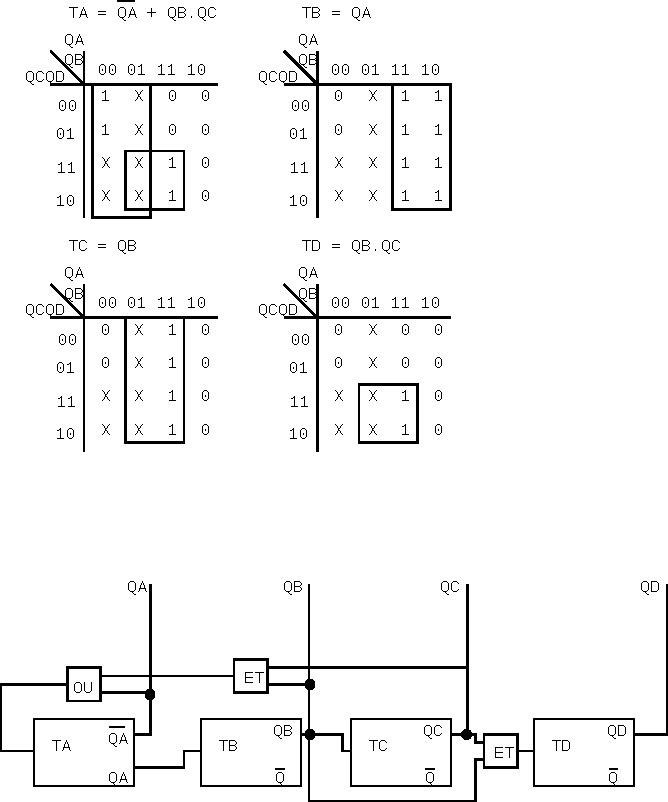
\includegraphics{TD8-compt}


        \end{solution}
      \item en utilisant des bascules JK.

        \begin{solution}
          Même méthode.
        \end{solution}
    \end{itemize}
\end{enumerate}

\section{Conversion série-parallèle}
\begin{center}
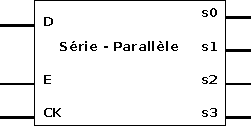
\includegraphics[width=3cm]{TD8-SP}
\end{center}

Un convertisseur série-parallèle possède trois entrées: $D$, $E$, et
un signal d'horloge $CK$. Il possède quatre sorties : les bits du mot $S$.

  Le convertisseur possède deux modes de fonctionnement:
  \begin{itemize}
  \item si $E=1$ alors à chaque front d'horloge le convertisseur lit la valeur
    de $D$. La sortie S est indéterminée.
  \item si $E=0$ alors la sortie S prend les 4 dernierès valeurs lues sur $D$.
  \end{itemize}


\begin{enumerate}
\item À partir d'une bascule D, concevez une bascule GL avec horloge
  (cf. question 2.3), composée de trois entrées $G,L,CK$ et de deux sorties $Q,
  \overline{Q}$. La bascule GL possède deux modes de fonctionnement:
  \begin{itemize}
    \item Si $G=1$, la bascule GL se comporte comme une bascule D normale.
    \item Si $G=0$, la bascul
e GL gèle les sorties $Q$ et $\overline{Q}$ et
      ignore l'entrée $L$.
  \end{itemize}

\begin{solution}
  On écrit l'équation caractéristique de la bascule GL:
  $$ Q^+ = GL + \overline{G}Q $$

  On écrit l'équation caractéristique de la bascule D:
  $$ Q^+ = D $$

  On peut simplifier: $$ D = GL + \overline{G}Q$$

  Ce qui nous donne le circuit suivant:
  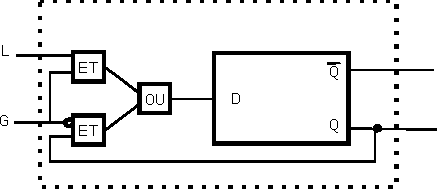
\includegraphics{TD8-GLD}
\end{solution}

\item À l'aide de bascules GL, concevez un convertisseur série-parallèle 4-bits.

\begin{solution}
  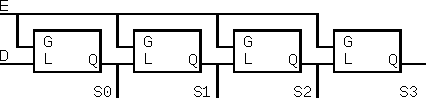
\includegraphics{TD8-seriepara}
\end{solution}
\item Concevez maintenant un convertisseur parallèle-série 4bits.
\begin{solution}
  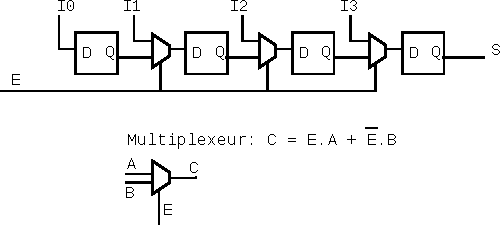
\includegraphics{TD8-paraserie}
\end{solution}


\end{enumerate}
\end{document}
